\documentclass{beamer}

\usepackage{tikzducks}
\usepackage{tikzlings}

\setbeamertemplate{navigation symbols}{}
\setbeamertemplate{background canvas}{
\includegraphics[height=\paperheight]{Background}}

\usepackage{xfp}
\ExplSyntaxOn
\let\intmodnn\int_mod:nn
\ExplSyntaxOff

\newcommand{\tourist}{%
\ifnum \intmodnn{\thepage}{10} > 5
	\mouse[
		rightstep,
		scale=1.6, 
		xshift=3cm, 
		yshift=-3.4cm,
		book={\tiny Guide},
		bookcolour=cyan!50!blue,		
	]
\else
	\mouse[
		leftstep,
		scale=1.6, 
		xshift=3cm, 
		yshift=-3.4cm,
		book={\tiny Guide},
		bookcolour=cyan!50!blue,		
	]
\fi
	\thing[
		scale=1.8, 
		xshift=3.17cm, 
		yshift=-3.15cm,
		strawhat=cyan!50!blue,
		ribbon=white!80!cyan,
		rotate=15
	]
}

\begin{document}

\begin{frame}
\begin{tikzpicture}[remember picture, overlay]
\node at (30-0.15*\thepage,0.4) {\includegraphics[height=5cm]{LastSupper}};
\node at (30-0.15*\thepage,-0.4) {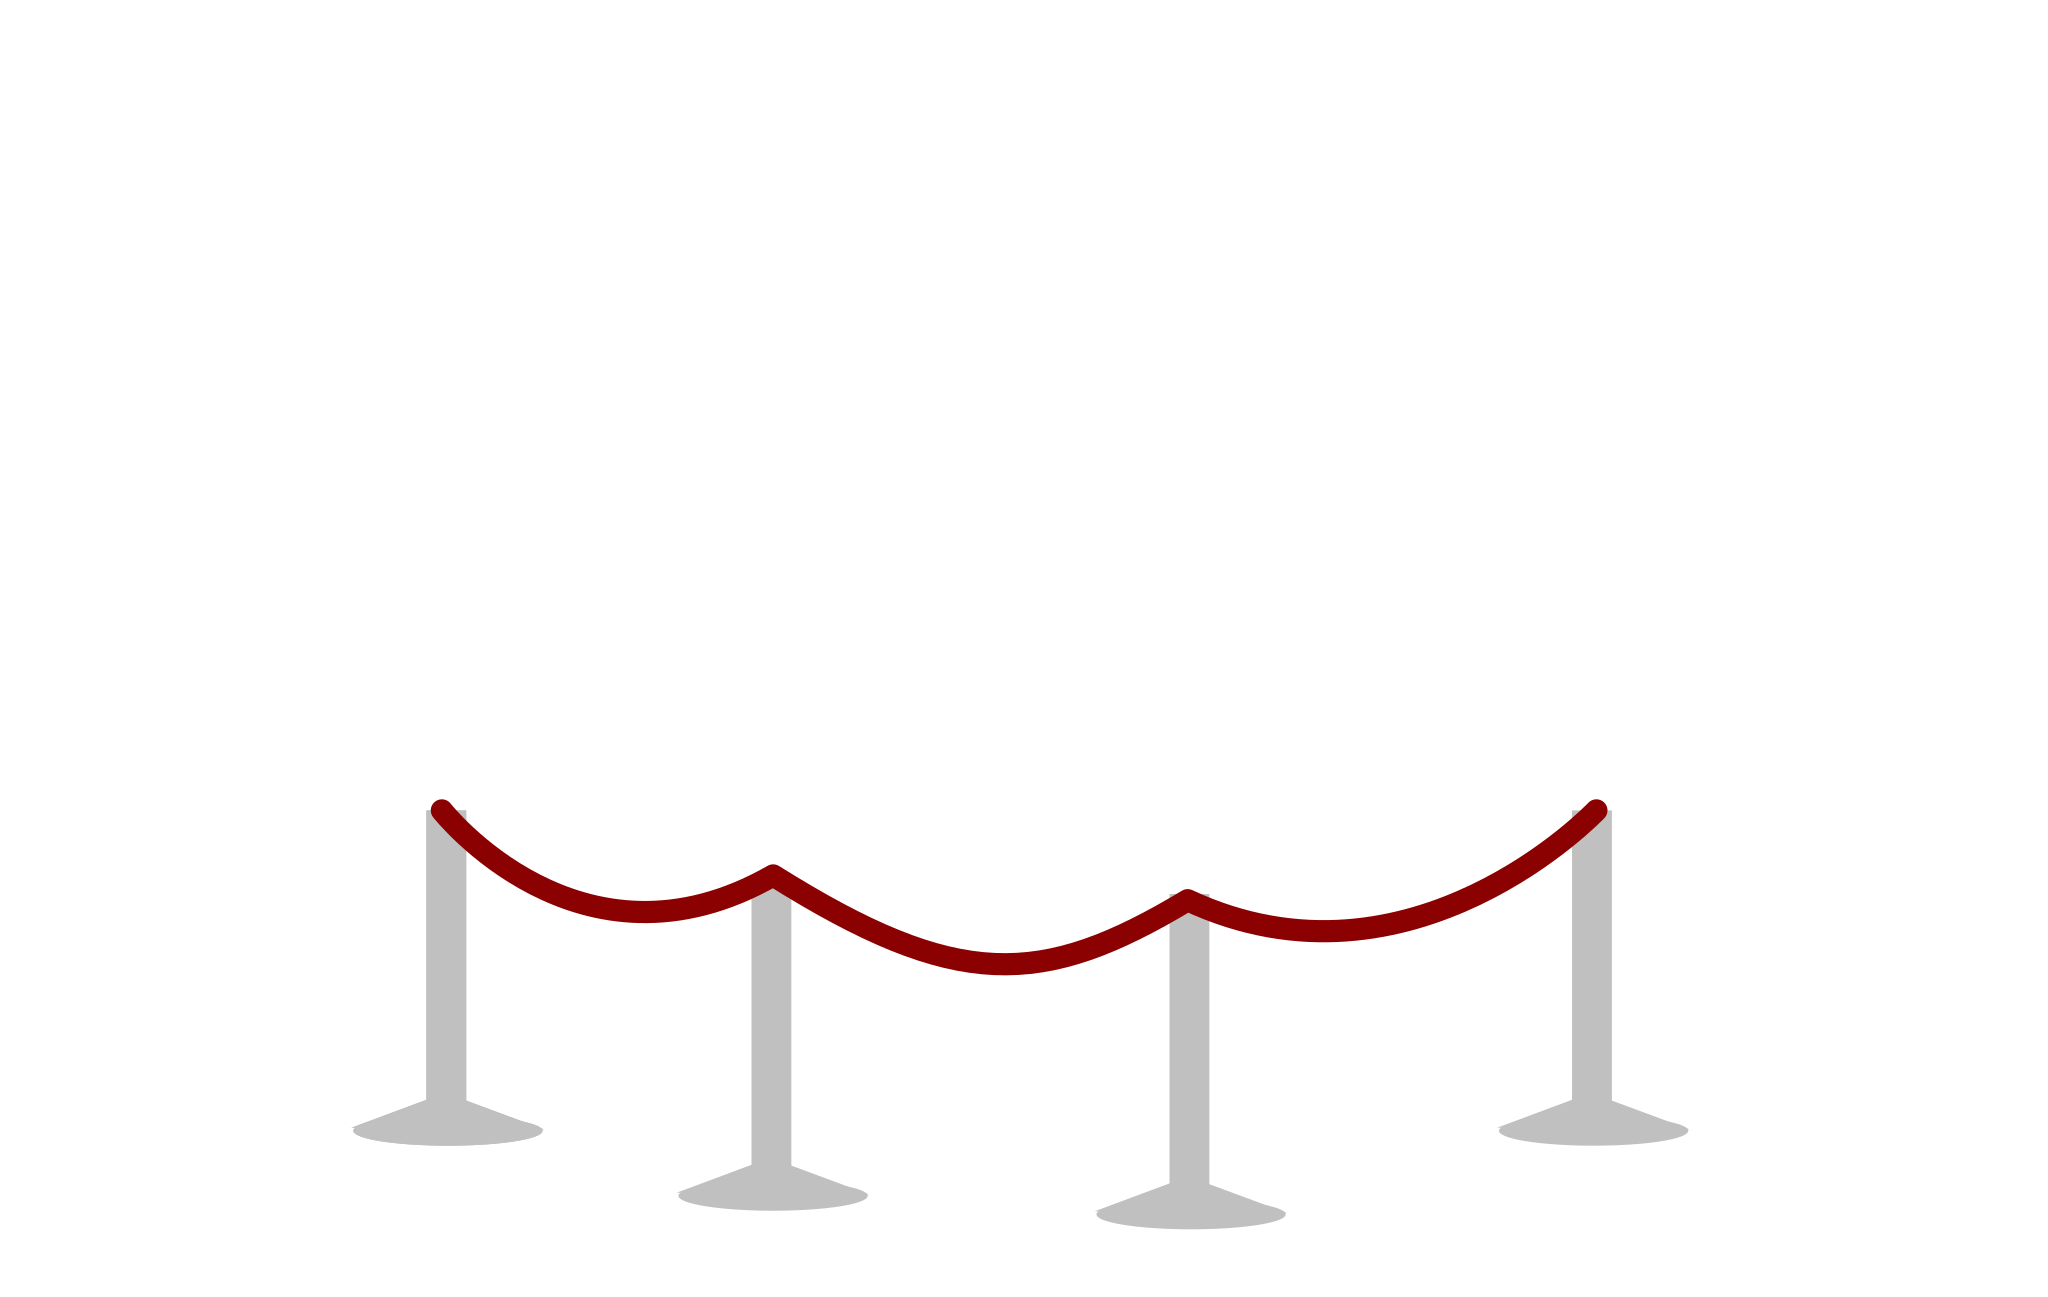
\includegraphics[height=\paperheight]{rail}};
\node at (50-0.15*\thepage,0.4) {\includegraphics[height=5cm]{ElGreco}};
\node at (60-0.15*\thepage,-0.4) {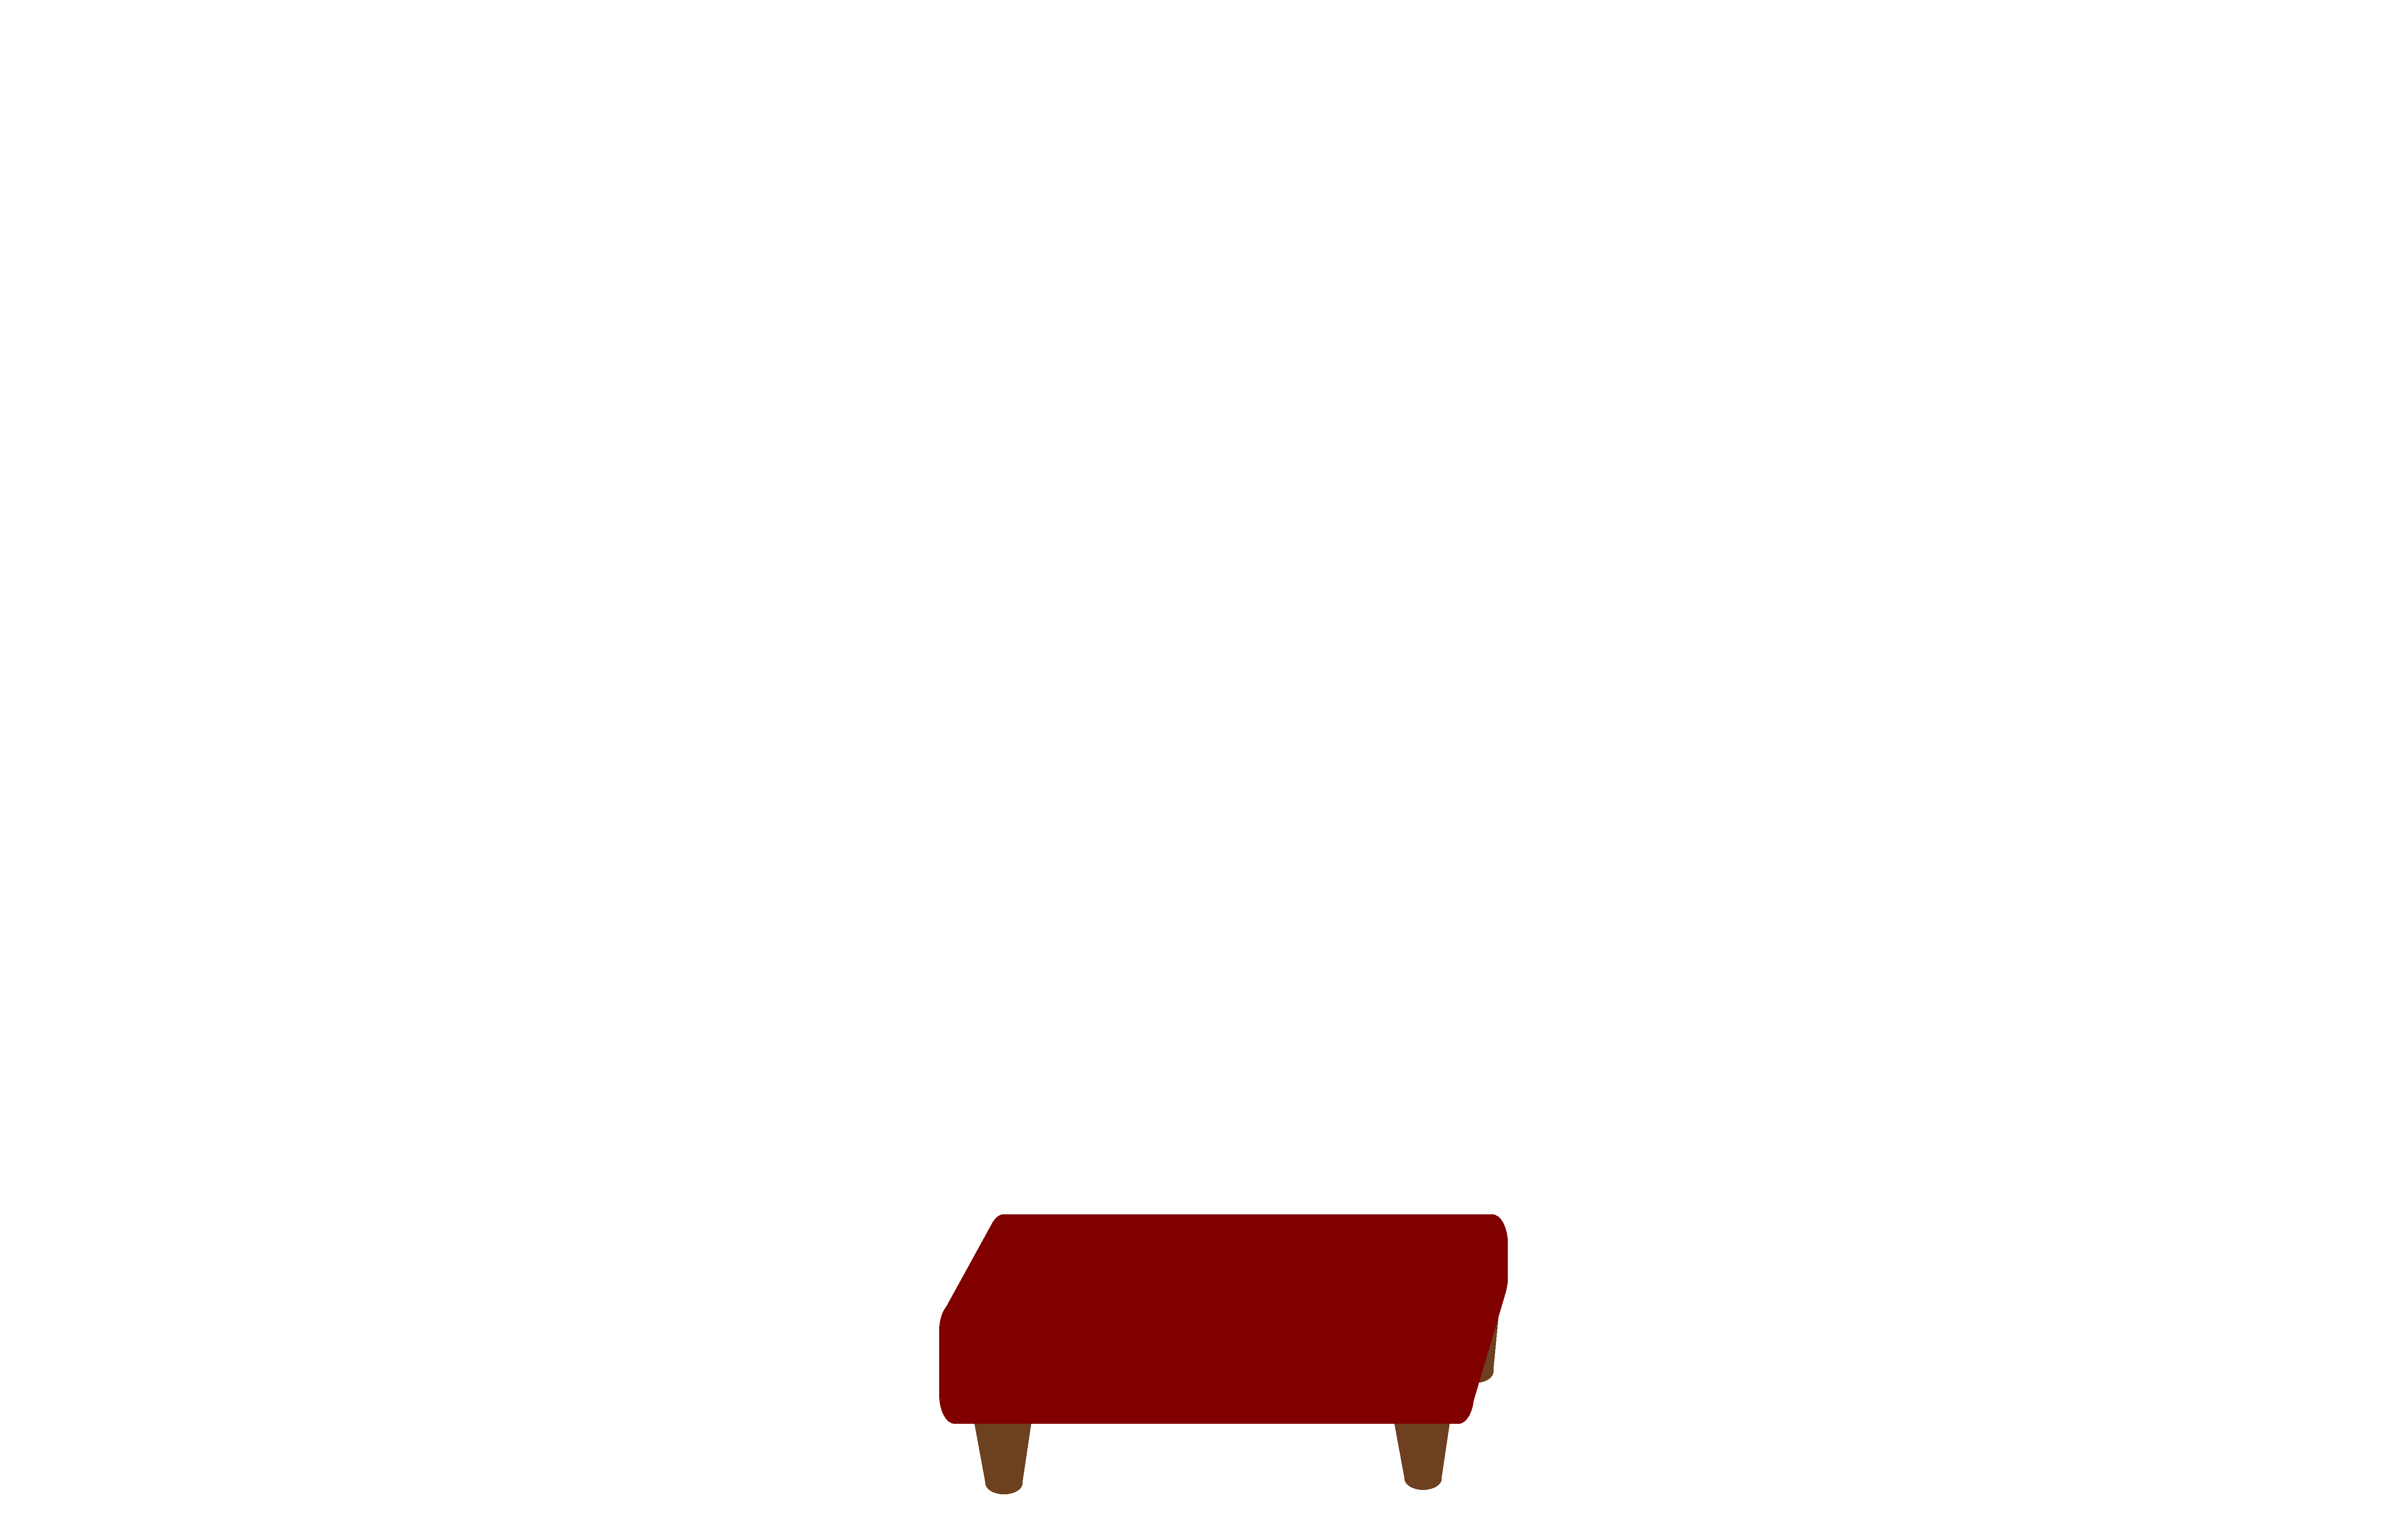
\includegraphics[height=\paperheight]{sofa}};
\node at (70-0.15*\thepage,0.4) {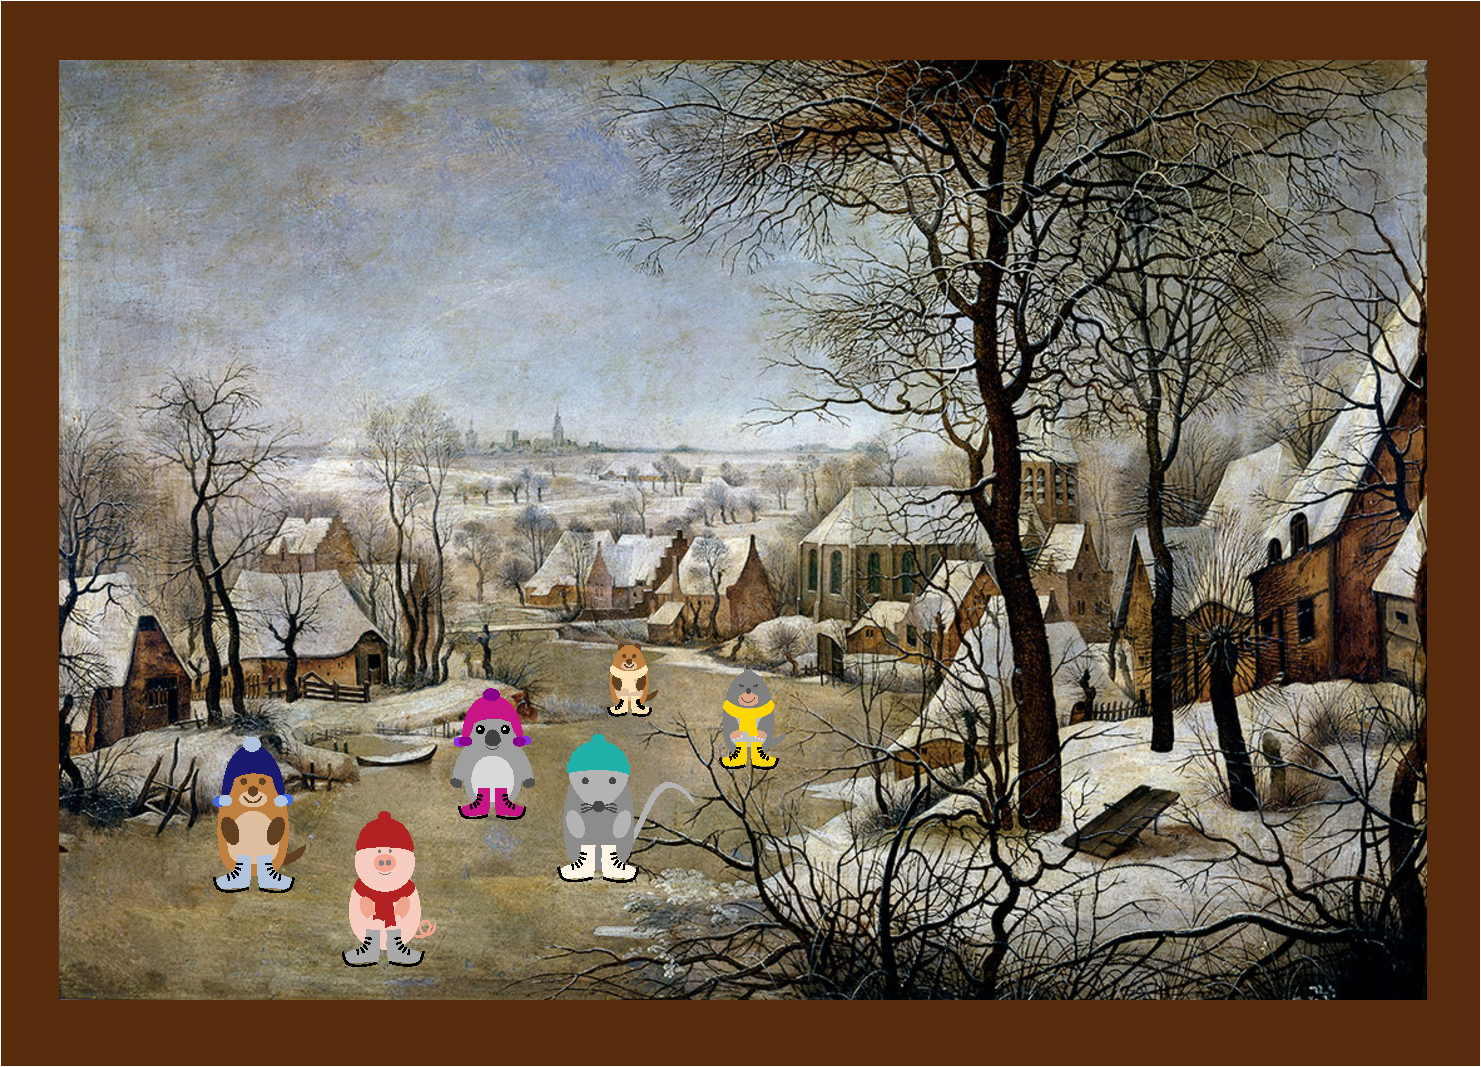
\includegraphics[height=5cm]{bruegel}};
\node at (90-0.15*\thepage,0.4) {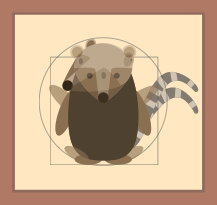
\includegraphics[height=5cm]{VitruvianCoati.png}};
\node at (90-0.15*\thepage,-0.4) {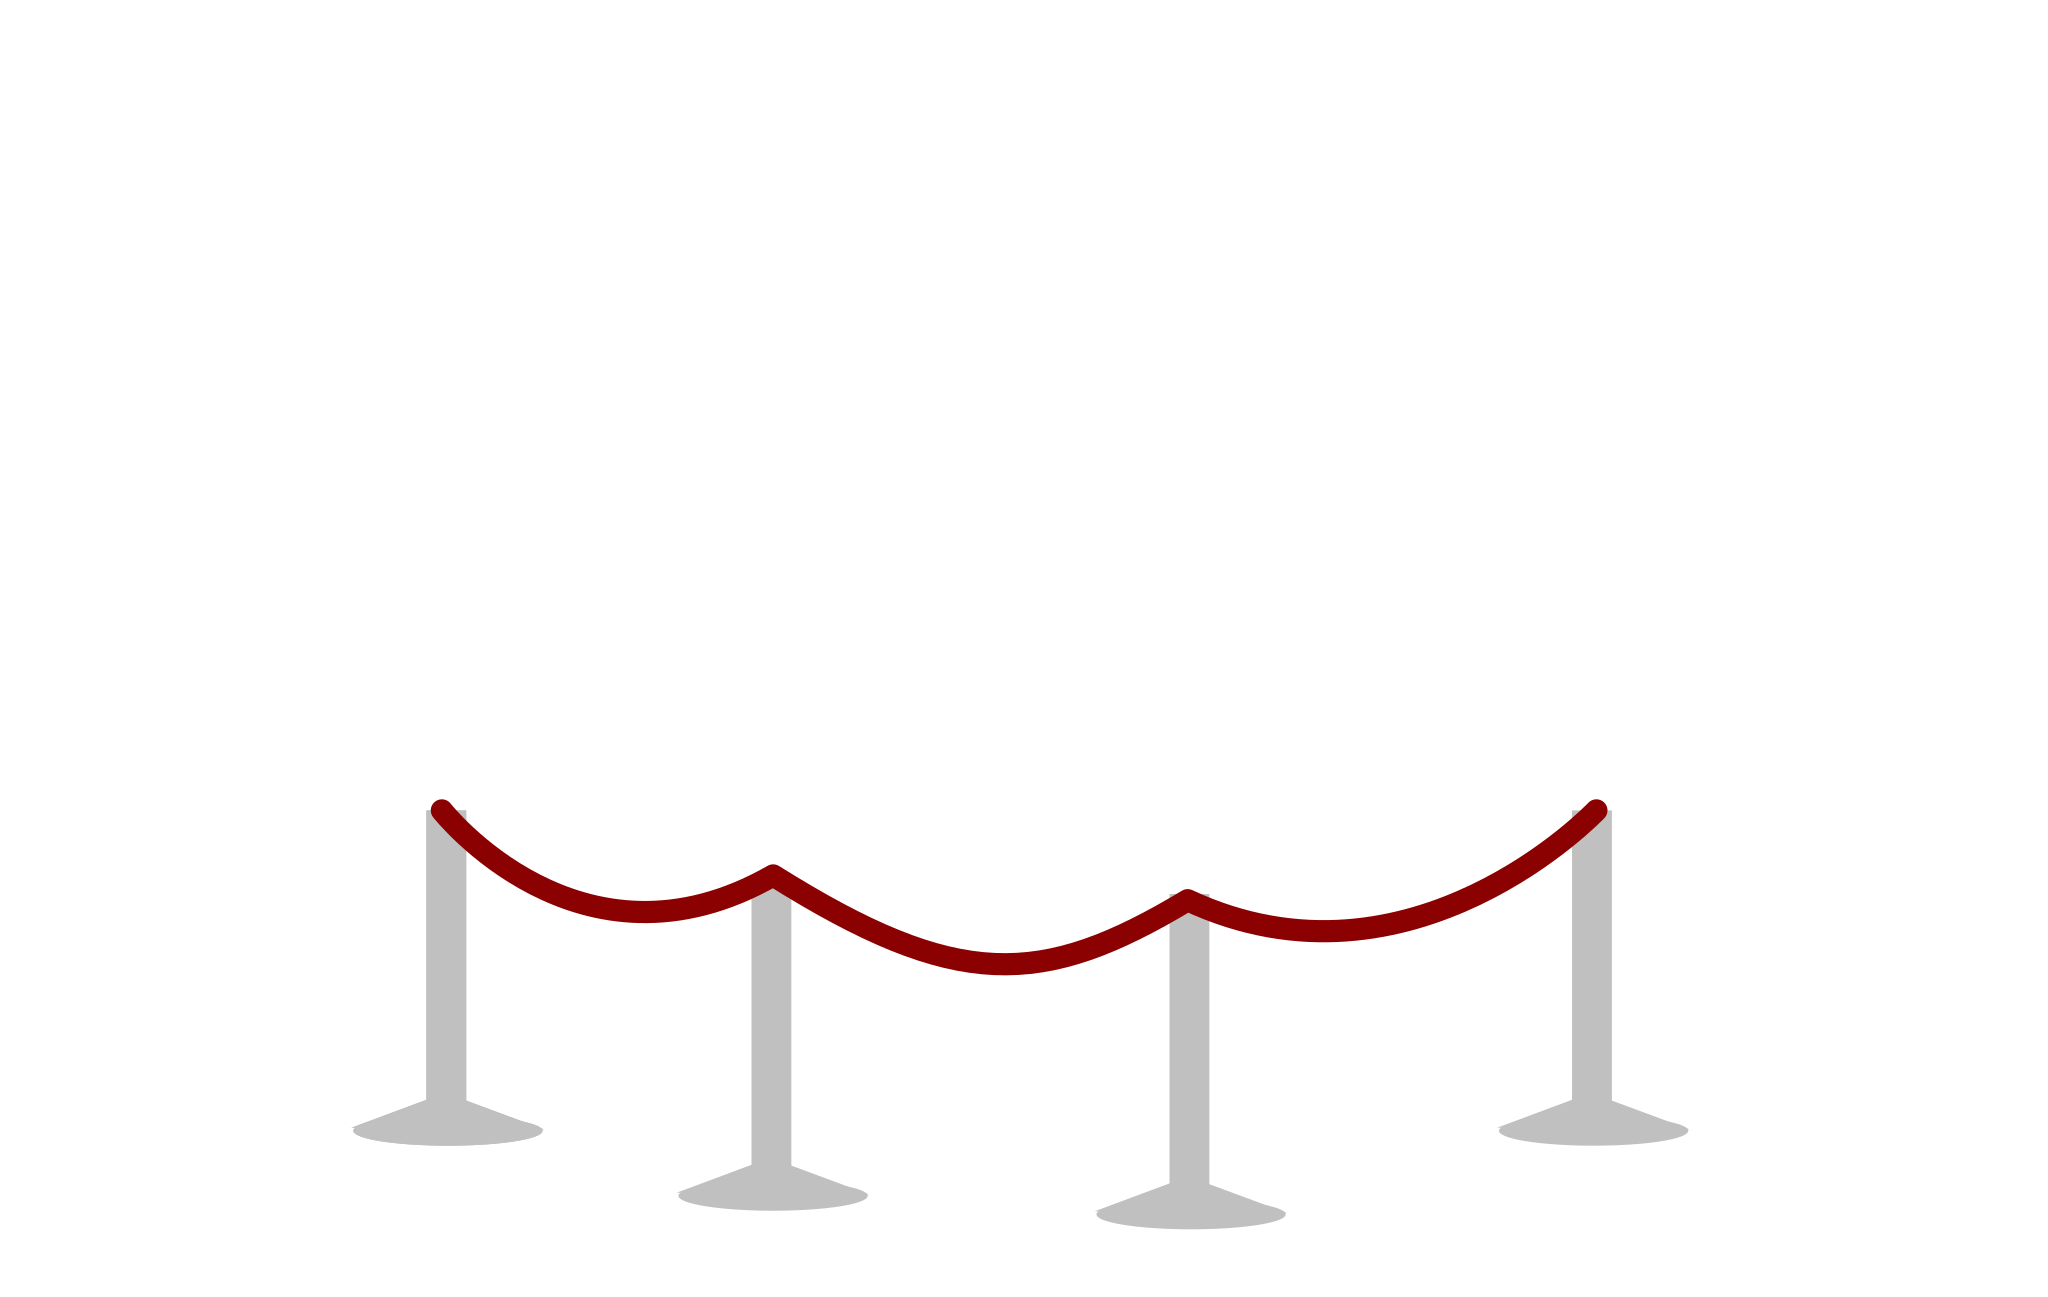
\includegraphics[height=\paperheight]{rail}};
\node at (110-0.15*\thepage,0.4) {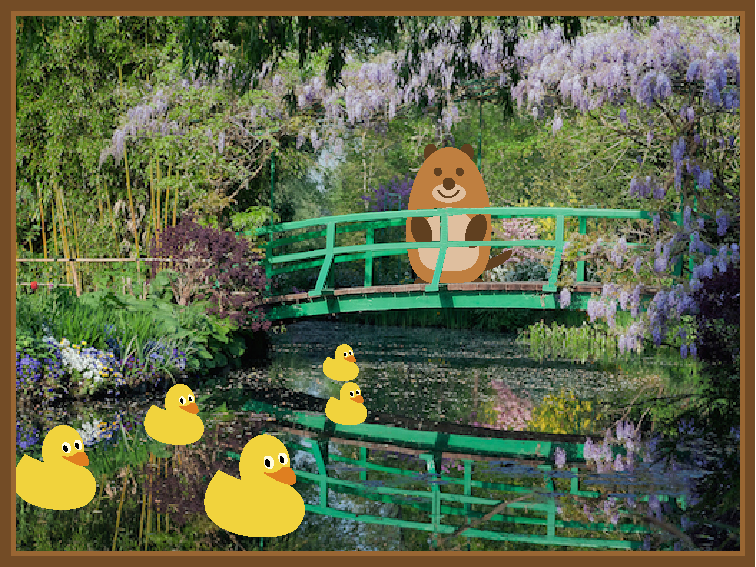
\includegraphics[height=5cm]{Monet}};
\node at (120-0.15*\thepage,-0.4) {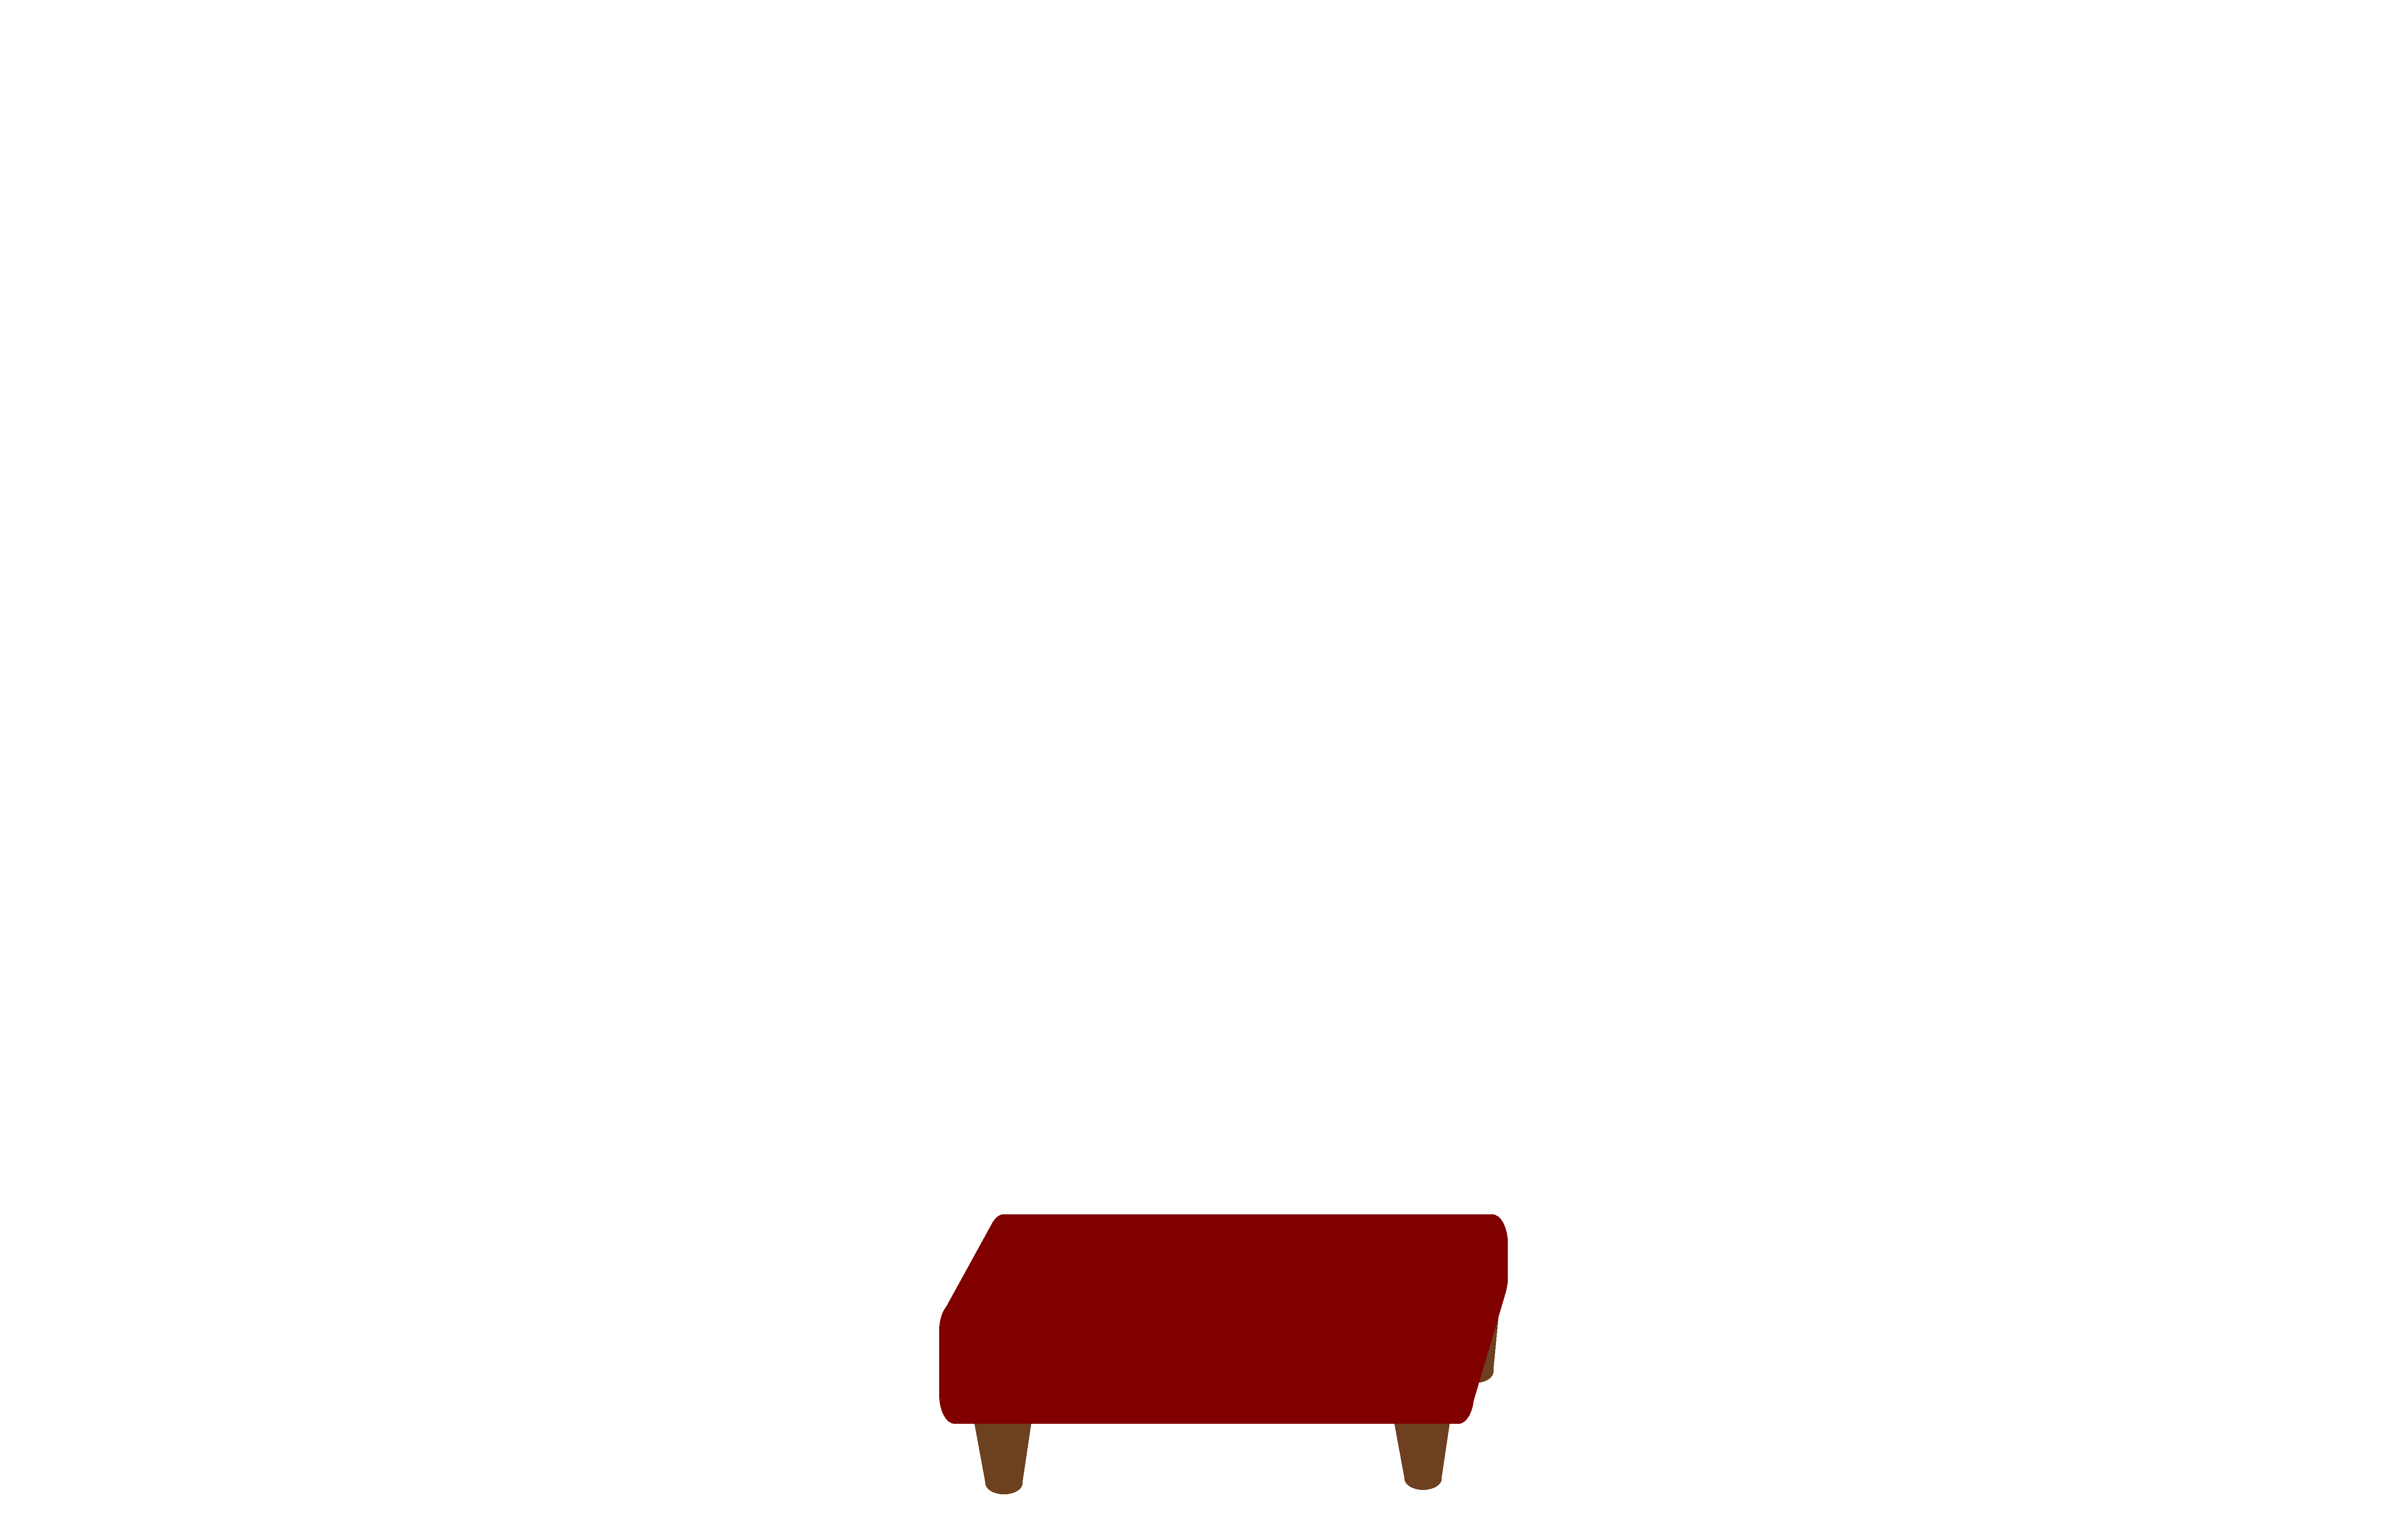
\includegraphics[height=\paperheight]{sofa}};
\node at (130-0.15*\thepage,0.4) {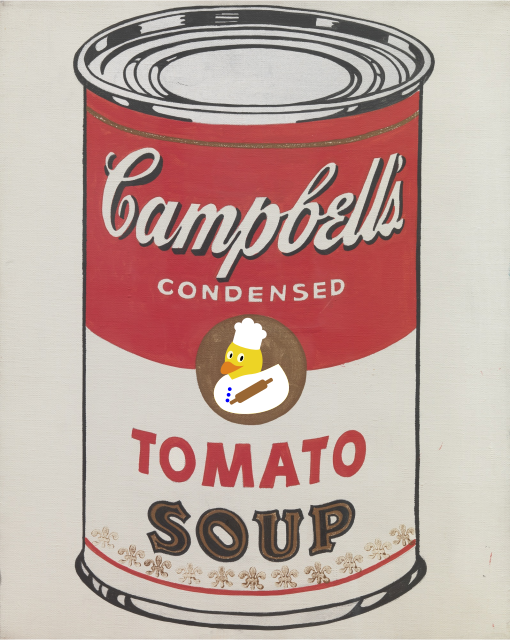
\includegraphics[height=5cm]{soup}};
\tourist
\end{tikzpicture}
\pause[930]
\end{frame}
	
\end{document}